\documentclass{article}
\usepackage{tikz}
\usetikzlibrary{matrix,arrows,decorations.pathmorphing,positioning}
\begin{document}

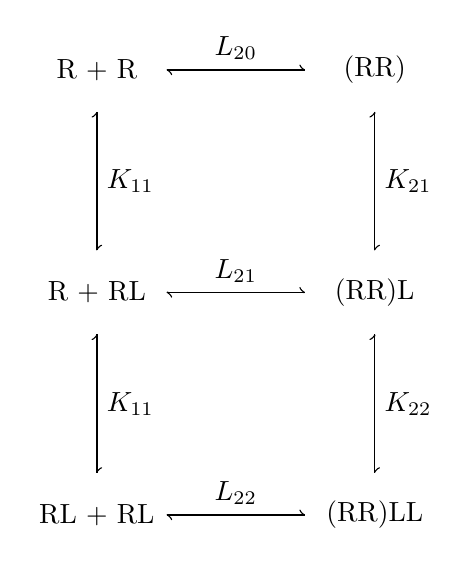
\begin{tikzpicture}
%add "text width=5em" in [] for left align 
\tikzstyle{node}=[minimum height=3em, minimum width=5em, node distance = 5em]
\node[node](A) at (0,0)  {R + R};
\node[node](B) [below = of A] {R + RL};
\node[node](C) [below = of B]  {RL + RL};
\node[node](D) [right = of A] {(RR)};
\node[node](E) [below = of D] {(RR)L};
\node[node](F) [below = of E]  {(RR)LL};
\draw[-left to, line width=0.5pt] (A) -- node[right]{$K_{11}$} (B);
\draw[-left to, line width=0.5pt] (B) -- (A);
\draw[-left to, line width=0.5pt] (B) -- node[right]{$K_{11}$} (C);
\draw[-left to, line width=0.5pt] (C) -- (B);
\draw[-left to, line width=0.5pt] (A) -- node[above]{$L_{20}$} (D);
\draw[-left to, line width=0.5pt] (D) -- (A);
\draw[-left to, line width=0.5pt] (B) -- node[above]{$L_{21}$} (E);
\draw[-left to, line width=0.5pt] (E) -- (B);
\draw[-left to, line width=0.5pt] (C) -- node[above]{$L_{22}$} (F);
\draw[-left to, line width=0.5pt] (F) -- (C);
\draw[-left to, line width=0.5pt] (D) -- node[right]{$K_{21}$} (E);
\draw[-left to, line width=0.5pt] (E) -- (D);
\draw[-left to, line width=0.5pt] (E) -- node[right]{$K_{22}$} (F);
\draw[-left to, line width=0.5pt] (F) -- (E);
\end{tikzpicture}
\\
\\
\\
\\
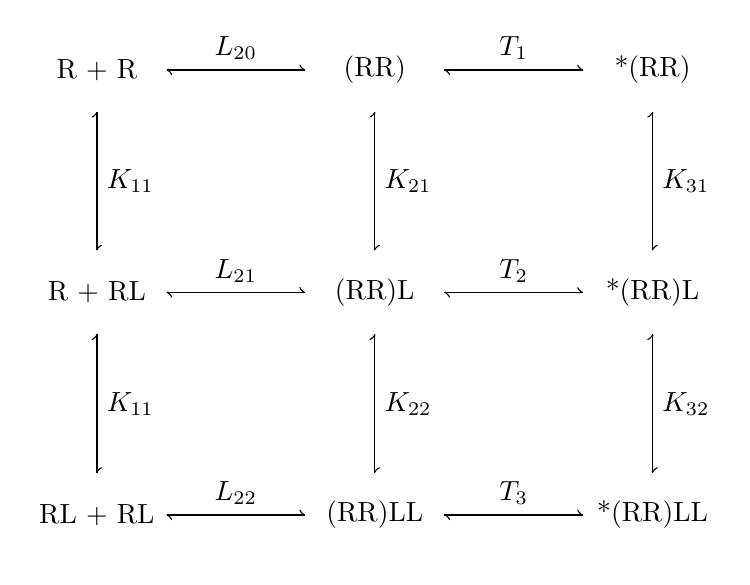
\begin{tikzpicture}
%add "text width=5em" in [] for left align 
\tikzstyle{node}=[minimum height=3em, minimum width=5em, node distance = 5em]
\node[node](A) at (0,0)  {R + R};
\node[node](B) [below = of A] {R + RL};
\node[node](C) [below = of B]  {RL + RL};
\node[node](D) [right = of A] {(RR)};
\node[node](E) [below = of D] {(RR)L};
\node[node](F) [below = of E]  {(RR)LL};
\node[node](G) [right = of D] {*(RR)};
\node[node](H) [right = of E] {*(RR)L};
\node[node](I) [right = of F]  {*(RR)LL};
\draw[-left to, line width=0.5pt] (A) -- node[right]{$K_{11}$} (B);
\draw[-left to, line width=0.5pt] (B) -- (A);
\draw[-left to, line width=0.5pt] (B) -- node[right]{$K_{11}$} (C);
\draw[-left to, line width=0.5pt] (C) -- (B);
\draw[-left to, line width=0.5pt] (A) -- node[above]{$L_{20}$} (D);
\draw[-left to, line width=0.5pt] (D) -- (A);
\draw[-left to, line width=0.5pt] (B) -- node[above]{$L_{21}$} (E);
\draw[-left to, line width=0.5pt] (E) -- (B);
\draw[-left to, line width=0.5pt] (C) -- node[above]{$L_{22}$} (F);
\draw[-left to, line width=0.5pt] (F) -- (C);
\draw[-left to, line width=0.5pt] (D) -- node[right]{$K_{21}$} (E);
\draw[-left to, line width=0.5pt] (E) -- (D);
\draw[-left to, line width=0.5pt] (E) -- node[right]{$K_{22}$} (F);
\draw[-left to, line width=0.5pt] (F) -- (E);
\draw[-left to, line width=0.5pt] (D) -- node[above]{$T_1$} (G);
\draw[-left to, line width=0.5pt] (G) -- (D);
\draw[-left to, line width=0.5pt] (E) -- node[above]{$T_2$} (H);
\draw[-left to, line width=0.5pt] (H) -- (E);
\draw[-left to, line width=0.5pt] (F) -- node[above]{$T_3$} (I);
\draw[-left to, line width=0.5pt] (I) -- (F);
\draw[-left to, line width=0.5pt] (G) -- node[right]{$K_{31}$} (H);
\draw[-left to, line width=0.5pt] (H) -- (G);
\draw[-left to, line width=0.5pt] (H) -- node[right]{$K_{32}$} (I);
\draw[-left to, line width=0.5pt] (I) -- (H);
\end{tikzpicture}

\end{document}